\chapter{Сокеты}

Абстракция сокетов введена в BSD (Berkeley Software Distribution) Unix. Сокеты создавались для организации взаимодействия процессов, причем безразлично, где они работают, на одной машине или на разных. Т.е. в распределенной системе, единообразно осуществляются взаимодейсвтие, будто менйфрейм или распределенная система. Сокеты представляют абстракцию конечной точки взаимодейсвтия. Процессы могут использовать единообразный интерфейс сокетов для отправки/получения сообщений (данных) как на локальной машине так и по сети, используя разные протоколы. 

Существует обобщенная иллюстрация, которая подчеркивает тот факт, что осуществляются соответствующие системные вызовы.

\lstinputlisting[language=c, caption = Создание сокета]{listing/6.c} 

\begin{figure}[H]
  \centering
  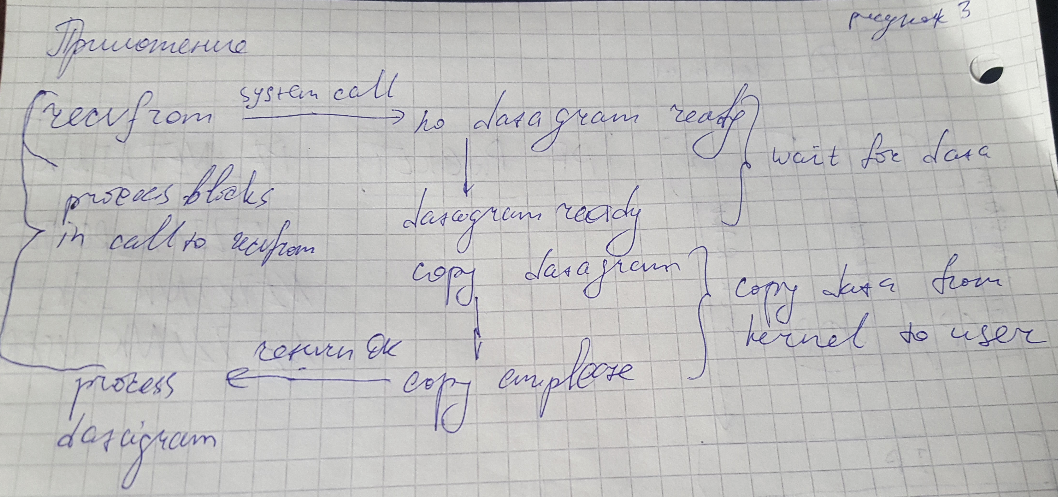
\includegraphics[width=\textwidth]{pic/1.png}
  \caption{Классификация}
  \label{pic_class_sockets}
\end{figure}

Пояснения к \ref{pic_class_sockets}:\\ 
\verb|PF_PACKET| - создано для непосредственного доступа приложений к сетевым ???. \\
\verb|NETLINK_##| - используются для обмена между пространством ядра и пространством пользователя.

Ядро линукс предоcтавляет для работы с сокетами один единственный системый вызов в $net/socket.c$

\lstinputlisting[language=c, caption = $sys\_socketcall$, label = code_sys_socketcall]{listing/1.c} 

Данная функция \ref{code_sys_socketcall} реализована как переключатель системных вызовов. 
call - типа int определяет номер нужной функции.

\lstinputlisting[language=c, caption = Номера call для старого ядра]{listing/2.c} 

Если функции \verb|sys_socket_call| передано параметр \verb|call = 1|, то будет осуществлен вызов \verb|sys_socket| (эта функция определена в файле $net/socket.c$ и в ней вызывается функция \verb|sock_create|) инициализирует структуру сокета \verb|struct_socket|

\lstinputlisting[language=c, caption = Структура сокет]{listing/3.c} 

Сокеты BSD следуют концепции UNIX. Все объекты с доступом чтения/записи отображены как файлы, чтобы можно было работать стандартными функциями. Объекты, которыми манипулируют при операции чтиения/записи в контексте транспортных протоколов являются конечные точки коммуникационных отношений (сокеты). 
Структура сокет содержит указатель на структуру $file$. 

Для сокета определено 5 состояний:
\begin{enumerate}
	\item \verb|SS_FREE| - не занят
	\item \verb|SS_UNCONNECTED| - не соединен
	\item \verb|SS_CONNECTING| - соединяется в данный момент
	\item \verb|SS_CONNECTED| - соединен
	\item \verb|SS_DISCONNECTING| - отсоединяется в данный момент
\end{enumerate}

Сокет является специальнеым файлом. Поэтому есть поле \verb|struct file| и оно ссылается на inode. 

\paragraph{Адреса сокетов}

Сокеты поддерживают множество протоколов, поэтому введена общая ??? $sockaddr$. При создании коммуникационных отношений необходимо указать адрес конечной точки коммуникационного партнера. 

\begin{lstlisting}[language=c, caption = Структура sockaddr]
struct sockaddr {
	//определяет семейство адресов
	sa_family_t sa_family;
	char sa_data[14]
}
\end{lstlisting}

Формат адреса подробно не определен, поэтому для адресов интернета используется другая структура \verb|sock_addr_in|:

\begin{lstlisting}[language=c]
#include </usr/include/netinet.in.h>
struct sockaddr_in {
	sa_family_t sin_family;
	unsigned short int sin_port;
	struct in_addr sin_addr;
	unsigned char sin_zero[sizeof(struct sockaddr) - sizeof(sa_family_t) - sizeof(uint16_t) - sizeof(struct in_addr)];
}
\end{lstlisting}

Адреса и номера портов должны быть указаны в сетевом порядке байтов. В сети и на компьютере может быть разный порядок байтов.

Сокеты в файловом пространстве имен. Это сокеты семейства UNIX. Тип DGRAM. Тут взаимодейсвтие осуществляется на локальной машине через файловое пространство имен. Создаем файл

\begin{lstlisting}[language=c]
//связываем с именем сокета.
strcpy(srvr_name,sa_data, "socket.soc");
\end{lstlisting}

Для семейства \verb|AF_UNIX| может использоваться только \verb|SOCK_DGRAM|. Для инернет домена могут использоваться \verb|SOCK_STREAM| и \verb|SOCK_DGRAM|. Для \verb|SOCK_RAW|  используются протоколы IP и ICMP и т.д.

Парные сокеты - сокеты в файловом пространстве имен. Для их создания используется функция 

\begin{lstlisting}[language=c]
socketpair(AF_UNIX, ..., 0, sockets)
//...
pid = fork () {...}

//sockets - массив из двух дескрипторов, также как в pipe. Уже готовы к передаче данных и можно сразу применять системные вызовы read/write. fork получает оба дескрпитора, один из которых он должен закрыть с помощью системного вызова close. Несмотря на то, что не используется модель клиент-сервер, которая характерная для сокетов, но если посомтреть, то функция socketpair получает семейство и тип, на основании которых определяется протокол, поэтому считаются полноценными сокетами. Это сделано для общности подхода реализации взаимодейсвтия через сокеты.
\end{lstlisting}

Сетевые сокеты, которые мы рассматривали \verb|AF_INET| и \verb|SOCK_STREAM|. Для них существует сетевой протокол.

Взаимодейсвтие процессов через сокеты идет по модели клиент-сервер, кроме парных сокетов, где по модели предок-потомок.

\begin{figure}[H]
  \centering
  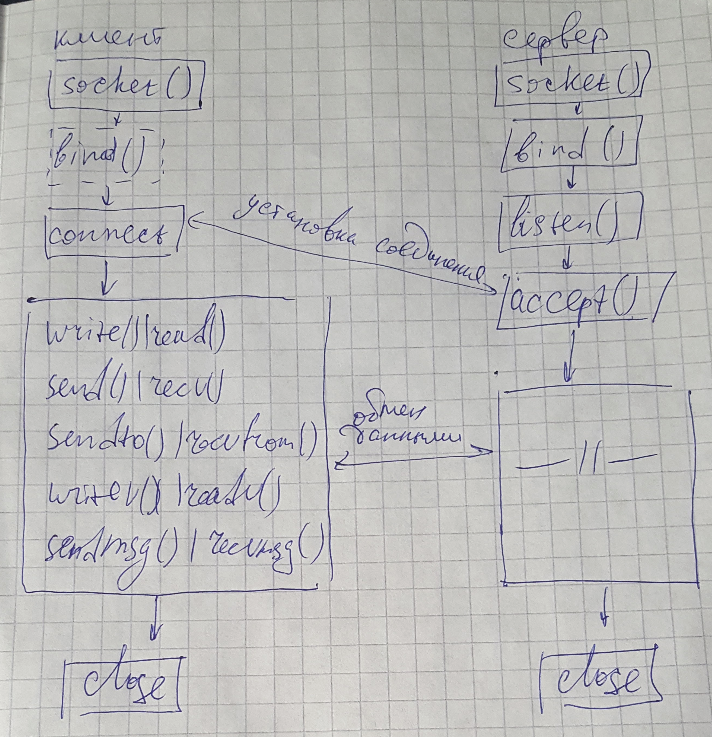
\includegraphics[width=\textwidth]{pic/2.png}
  \caption{pic}
  \label{pic_alhoritm_cs}
\end{figure}

Пояснения к \ref{pic_alhoritm_cs}:\\
Пунктир - не обязательно.\\
\verb|bind()| - для назначения сокету локального адреса. Для сокетов интернета этот адрес состоит из ip адреса сетевого интерфейса локальной системы и номера порта. Клиенты могу действовать без вызова bind так как их точный адрес не играет ни какой роли и в этом случае адрес назначается автоматически.\\
\verb|listen()| используется сервером для информирования операционной системы о том что в сокете нужно принять соединение. Очевидно это имеет смысл ориентированных на соединение (в настоящее время это только TCP)\\
\verb|connect()| - устанавливает соединение, например TCP по переданному адресу. Для протоколов без установления соединения (UDP) может использоваться для указания адреса назначения для всех передаваемых пакетов.\\
\verb|accept()| - используется сервером для принятия соединения при условии, что он ранее получил запрос на соединение. В противном случае вызов будет заблокрирован до тех пор, пока не поступит запрос соединения. Когда соединение принимается, сокет копируется, а именно первоначальный сокет остается в состоянии $listen$, а новый сокет в состянии $connected$.  Вызов $accept$ возвращает новый дескриптор файла для следующего сокета. Такое дублирование сокетов в ходе принятия соединения дает серверу возможность продолжить принимать соединения без необходимости предвариательно закрывать предыдущие соединения.

\chapter{Модели ввода-вывода}
Базовая информация в книге \cite{UNIX_Stiv_net_app}.
Еще информация есть на сайте \cite{IBM_models_io}.

\begin{table}[H]
\begin{tabular}{|l|l|l|}
\hline
- & блокирующий & неблокирующий\\
\hline
синхронный & read/write & read/write (O\_NONBLOCK)\\
\hline
асинхронный & i/o multiplexing (select/poll) & AIO\\
\hline
\end{tabular}
\end{table}

Синхронное-Блокирующее: ??? процесс разблокируется и процесс в результате премещения данных из ядра в соответсвующий буфер. Один из видов buttom half - завершение прерывание, посылка данных куда надо и процесс разблокируется. 

Картинка первая модель блокирующий ввод/вывод. По всем канонам является синхронным. 

\begin{figure}[H]
  \centering
  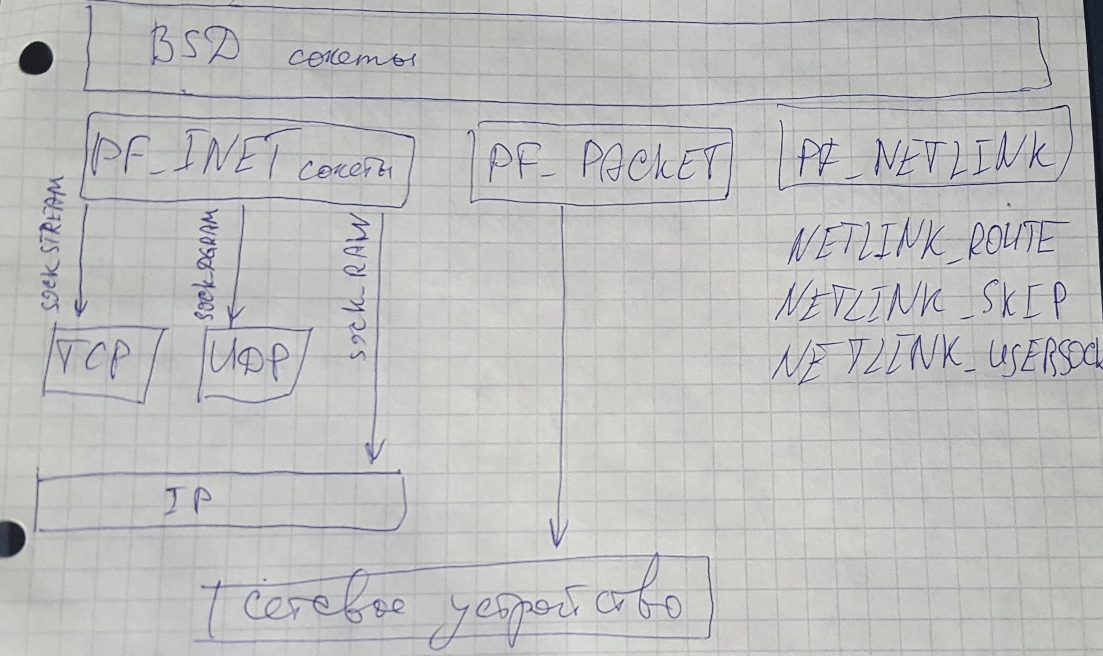
\includegraphics[width=\textwidth]{pic/3.png}
  \caption{pic}
\end{figure}

Все модели ввода/вывода в \cite{UNIX_Stiv_net_app} привязаны к сокетам.

Замечания к моделям ввода/вывода:
\begin{enumerate}
	\item \textbf{модель №2}: неблокирующий ввод вывод. Это синхронная модель. Связана эта модель с опросом polling. В соответствии с этой моделью, процесс выполняет системный вызов многократно. Это менее эффективный вариант синхронной блокировки, можно сказать, что это синхронный не блокирующий ввод/вывод. Очевидно, операция запрос ввода/вывода не может быть удовлетворен немедленно, и возвращается ошибка, что приводит к повторному запросу. Процесс вынужден многократно выполнять запросы, чтобы получить нужные данные.

	\item \textbf{модель №3}: с мультиплексированием - ассинхронная блокирующая. Процесс блокируется на мультиплексере.  

	\item \textbf{модель №3А}: модель похожая на мультиплексирование, но связана с созданием потоков(thread) каждый поток блокируется, но блокируется только один поток. Это дорогой путь.

	\item \textbf{модель №4}: ввод/вывод управляемые сигналы SIGIO. Это асинхронный и рассматривается он как неблокирующий. В \cite{UNIX_Stiv_net_app} подчеркивается, что процесс блокируется, пока данные блокируются в проложение. Информирование процессов управляется сигналами, пока сигнал не получен, процесс может выполнять вскую работу.

	\item \textbf{модель №5}: асинхронный не блокирующий. Асинхронный - это когда инфомирование приходит не зависимо от того, что в данный момент процесс выполняет. Все сигналы - асинхронные события, так же как и прерывания и связаны с прерываниями. СОоответственно смысл неблокирования в том, что процесс заинтересован в получении данных, он может обрабатывать большое колличества данных. Для увелечения эффективности, хорошо, при обработке одних данных, получать другие данные.
\end{enumerate}

Есть статья \cite{David_async},где рассматривают сигналы и асихронщину с другой точки зрения, и в конце говорит, что это "сложно и плохо".
